
\vspace{1cm}

\section{Concepts}

\subsection{Introduction}

Un web Service Composite est  le résultat des différentes combinaisons de plusieurs web Services qui vise à répondre aux requêtes complexes des utilisateurs.
Pendant l'exécution des Web services composites (CWS), un Web service composant (WS) peut échouer ou tomber en panne, et pour cela il existe des stratégies qui permettent la réparation du problème telles que  la réexécution du WS,la réplication,Récupération arrière ou point de contrôle.
La question qui se pose, quelle est la meilleure stratégie de récupération ? 
( a revoir ) 

\subsection{Web Service Composite}

L'architecture orientée services ( SOA Services Oriented Architecture) est une architecture logicielle qui met en oeuvre un ensemble de services simples (Composants logiciels).

L'architecture orientée services a pour objectif la décomposition d'une fonctionnalité en un ensemble de fonctions basiques, appelées services, fournies par des composants et la description des interactions entre ces services.


\begin{figure}[H]
\begin{center}
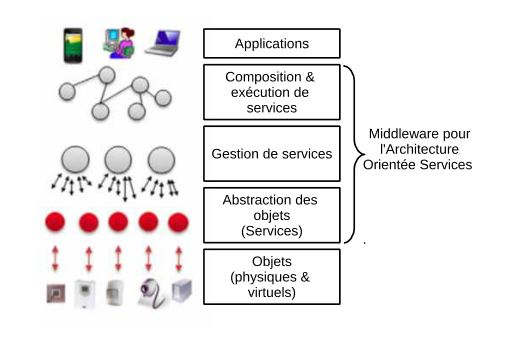
\includegraphics[width=1\linewidth]{images/Middleware SOA.jpg}
\end{center}
\caption{Middleware pour l’Architecture Orientée Services}
\label{fig:1}
\end{figure}

La figure 1 illustre l'architecture orientée services, la contribution de ce mémoire se positionne dans la couche Composition et exécution de services.
Cette couche fournit une composition des services et se charge du suivi de l’exécution de ces services composites. Un aspect important de cette couche est la résilience aux
pannes et l’adaptation en fonction des changements dans le système [Rafael Enrique Angarita Arocha].



D'après l'architecture vu précédemment, Un service Web composite peut être définis comme un  résultat d’une composition de plusieurs Web services, et qui peut à son tour entrer dans une autre composition.
Les  services web composites ont pour objectif  la production des services complexes pour répondre à des demandes d’utilisateurs complexes. 

La structure d’un Web service composite peut être générée manuellement ou automatiquement. Selon les requêtes demandées, les utilisateurs peuvent spécifier manuellement comment les fonctionnalités des Web service seront combinées ou bien  un composeur qui prend la responsabilité d’une génération automatique des Web service Composite en fonction de la demande, pour qu’ils seront finalement exécuté par un moteur d’exécution.


\begin{figure}[H]
\begin{center}
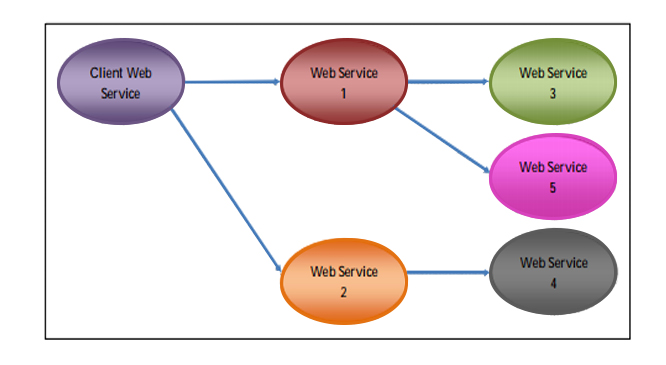
\includegraphics[width=1\linewidth]{images/CWS.jpg}
\end{center}
\caption{Web service composite}
\label{fig:2}
\end{figure}



Les Web services composite peuvent être représentés sous différents formes et structures en indiquant l’ensemble des informations et instructions relatives, comme l’ordre d’exécution et le comportement des Web services composants ainsi que les flux de données  et de contrôle.
La représentation peut être sous forme de Workflows, Graph ou réseau de Petri.



Les différents travaux et articles scientifiques sur la composition des services Web considèrent la composition de services Web comme étant un moyen efficace 
pour créer, exécuter, et maintenir des services qui dépendent d’autres services. Les auteurs ont défini le cycle de vie d’une composition de services Web reposant à partir de six activités [Benatalla] [Céline Lopez-Velasco]: 

- L’encapsulation de services natifs (Wrapping services): Cette première activité permet de  s’assurer que tout service peut être appelé lors d’ une composition, indépendamment de son  modèle de données, de son format de message, et de son protocole d’interaction. 


- L’établissement d’accord d’externalisation (Setting outsourcing agreements): Cette seconde activité consiste à négocier, établir, et appliquer des obligations contractuelles entre les services.


- L’assemblage de services composants (Assembling composite services):Cette activité permet  de spécifier, à un haut niveau d’abstraction, l’ensemble des services à composer afin d’atteindre  l’objectif attendu. Cet assemblage comporte une phase d’identification des services et de spécification de leurs interactions conformément aux descriptions et aux accords entre services. 


- L’exécution de services composants (Executing services):Cette activité consiste en l’exécution des spécifications de la composition précédemment définies. 


- Le contrôle de l’exécution de services composites (Monitoring services): La phase de contrôle permet de superviser l’exécution de la composition en vérifiant, par exemple, l’accès aux services, les changements de statut, les échanges de messages. Ce contrôle permet de détecter des violations de contrats, de mesurer les performances des services appelés et de prédire des exceptions. 


- L’évolutivité des services (Evolving services):Cette dernière phase permet de faire évoluer la composition en modifiant les altérations de l’organisation de services, en utilisant de nouveaux  services, ou en prenant en compte les retours de la phase de contrôle. 
[Céline Lopez-Velasco]



Dans ce mémoire, nous considérons les services avec leurs définition général c'est à dire des opérations exposées
sur Internet qui sont indépendantes de leur mise en œuvre. les détails d’implémentations telles que SOAP ou REST sont hors du domaine d’investigation de ce mémoire.

Les services sont décrits en fonction de leur fonctionnalités et des critères de qualité de service (QoS). Dans notre cas, la fonctionnalité d’un service est donnée par les paramètres d’entrée et de sortie.

\subsubsection { Qualité de Service }

La qualité de service (QoS Quality of Service) décrivent les caractéristiques non fonctionnelles du service Web, autrement dits la mesures dans laquelle un ensemble de caractéristiques répond à un besoin ou une attente.

nous considérons les trois critères de qualité suivantes [Rafael Enrique Angarita Arocha] :

- Temps de réponse: le temps estimé nécessaire pour achever une invocation de service ; qui est, la durée entre une demande de service et la réponse du service correspondant.

- Disponibilité : la probabilité d’obtenir une réponse correcte après une invocation de service. Cela inclut la probabilité que le service est disponible, qu’il s’exécute correctement, et que la transmission de message entre le
service et le demandeur a réussi.
 
- Prix: une mesure du coût d’exécution d’un service.


\subsection{Exécution tolérante aux pannes}

La tolérance aux pannes est la manière dont un système informatique, un système électronique ou un réseau répond à une défaillance matérielle ou logicielle. Le terme fait essentiellement référence à la capacité d'un système à prendre en compte les défaillances ou les dysfonctionnements d’un ou de plusieurs de ses composants, tout en fournissant un service ininterrompu, et cette capacité peut être fournie par un logiciel, un matériel ou une combinaison des deux.

Le but est d'éviter une panne catastrophique qui pourrait résulter d'un seul point de défaillance. 

\subsubsection{Défaillance des Web Service Composite}

Comme toutes les technologie, Les Web services Composite ne peuvent pas s’échapper aux défaillances d’exécution à 100 \%, car des pannes peuvent survenir à tout moment au niveau du matériel, du moteur d’exécution ou tout simplement du défaillance d’un Web service composant.
Cependant les Web Services Composite fonctionne potentiellement de manière réduite (en mode dégradé).


Soulever et relever les défis posés par les problématiques de résilience et de fiabilité des web services composite nécessite en premier lieu l’analyse  des caractéristiques des pannes dans  leur exécution.
On peut distinguer principalement dans l’environnement d’exécution des Web services Composites deux classe de pannes. 

    - Panne de nature silencieuse: (silent faults) Sont les pannes indétectables, ou qui sont détectées après une très grande durée depuis leurs déclenchements ce qui implique nécessairement que le résultat fourni est incorrect. 
    Ces pannes sont génériques pour tous les WS. Ils empêchent les WS de répondre.


    - Panne de nature logique: (Logic fault): Contrairement au pannes silencieuse, les panne logiques sont spécifiques aux différents Web service, et les attributs des entrées représente la cause principale de ces pannes.
    Ce genre d’erreur est difficile d’être identifié par le moteur d’exécution des Web services composites.

\subsubsection{Exécution tolérante aux pannes des CWS}

Le contrôle d'exécution des Web services composites peut être centralisé c’est à dire un coordinateur qui va jouer le rôle de la gestion de toute l’exécution,  ou distribué dans lequel le processus d’exécution de déroule avec la collaboration de plusieurs participants sans un coordinateur central. Comme il peut être attaché aux web services composants ou indépendant.
Certaines méthodes indépendantes de tolérance aux pannes dont apparus, telles que les propriétés transactionnelles et la réplication. Les propriétés transactionnelles décrivent implicitement le comportement des services web en cas d'échec, et sont utilisées pour garantir la propriété transactionnelle d’atomicité.

Les propriétés transactionnelles les plus utilisées pour les services web sont pivot, compensable, et retriable [Rafael Enrique Angarita Arocha],[modeling dinamic ...] \cite{1}. 
 
 - Pivot(p) : un service est appelé pivot si ses effets restent pour toujours
et ne peuvent pas être annulés sémantiquement une fois qu’il a terminé son exécution avec succés. Il s’agit de la propriété transactionnelle la plus basique.

- Compensable (c) : un service est compensable s’il existe un autre service qui peut sémantiquement annuler son exécution s'il n'as pas pu terminer avec succès.  
 
- Retriable (r) : un service est retriable s’il garantit une exécution réussie après un nombre fini d’invocations. Cette propriété doit être combinée avec les propriétés pivot ou compensable, créant les propriétés pivot-retriable (pr) et compensable-retriable (cr).

Les services Web composites sont construit à partir d'un ensemble des service qui offrent des propriétés transactionnelles garantissent la cohérence su système et ont une propriété transactionnelle agrégée comme suit [Rafael Enrique Angarita Arocha]: 

- Atomique : un service composite est atomique si au moins un de ses services composant est pivot ou pivot retriable. Lorsqu’un service composite atomique se termine avec succès, ses effets demeurent pour toujours et ils ne peuvent pas être annulées. Si l’un de ses services composants tombe en panne, le système est laissé dans un état sémantiquement similaire à celui qu’il avait avant l’exécution du service composite.


- Compensable : un service composite est compensable si tous ses services composants sont compensables. Cela signifie qu’il existe un autre service composite, contenant les services qui compensent les services du service composite compensable, qui peut annuler sémantiquement les effets du service composite compensable après son exécution réussie. Comme pour le service composite atomique, si l’un de ses service composants tombe en panne, le système est laissé dans un état sémantiquement similaire à celui qu’il avait avant l’exécution du service composite compensable.


- Retriable : un service composite est retriable si tous ses services composants sont retriables. Un service composite retriable garantit l’exécution réussie après un laps de temps limité. Cette propriété doit être combinée avec les propriétés atomiques ou compensables, pour créer les propriétés atomique-retriable (ar) et compensable-retriable (cr).


\subsection{Mécanisme de récupération}

En présence des pannes, les propriétés transactionnelles fournis par les services ont une importance dans la création des services composites fiables, car ils assurent un état cohérent de l'ensemble du système.

La stratégie de reprise d'une exécution de service composite dépend de la propriété transactionnelle des services composants.
Les principaux mécanisme de récupération sont \cite{1} : 

- Récupération en arrière : c'est l'opération de restauration de l’état du système avant l’exécution du service composite ; c’est-à-dire, tous les effets produits par le service en panne sont annulées par rollback, et les effets des services exécutés avant la panne sont sémantiquement annulés en utilisant des techniques de compensation (Fig (a)).


- Récupération en avant : c'est l'opération qui permet la réparation du panne afin que le  service composite peut poursuivre son exécution ; les techniques utilisées pour fournir une récupération en avant sont le réessayage de l’invocation de service ou le remplacement du service (Fig (b)).


- Récupération sémantique : elle a le même mécanisme que la récupération en arrière, sauf que la récupération sémantique est effectuée après une exécution réussie d’un service composite en compensant l’exécution de ses services composants. L’idée est de laisser le système dans un état sémantiquement proche de l’état qu’il avait avant l’exécution du service composite (Fig (c))

- Checkpointing : c'est l'opération qui permet si une panne survient de continuer l’exécution de la partie du service composite qui n’a pas été affecté par cette panne, tout en retardant l’exécution de la partie affectée (Fig (d))

\begin{figure}[H]
\begin{center}
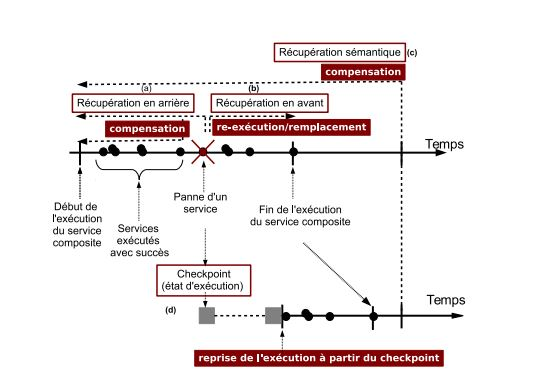
\includegraphics[width=1\linewidth]{images/techs reparation.jpg}
\end{center}
\caption{Stratégies de récupération \cite{1}}
\label{fig:3}
\end{figure}